\scanpage{49}
\mspage{48}
et par la condition (iv), il reste à vérifier que
\[
\overline{A}^{({\unsure{\mathcal{T}|\tau}}'')}\cap T\quad\text{est}\quad\mathcal{T}\text{ fermée}\quad ??
\]
% slanted
\margin{C'est peut-être faux ?}

C'est ultra faux \unsure{on voit|en voici|on va voir}

\diagram{\begin{tikzcd}[ampersand replacement=\&,column sep=2.05em,row sep=.75em,
execute at end picture={
\draw ([xshift=-9pt,yshift=5pt]u.center) .. controls ([xshift=-9pt,yshift=19pt]u.center) and ([xshift=4pt,yshift=30pt]u.center) .. ([xshift=20pt,yshift=31pt]u.center) .. controls ([xshift=10pt,yshift=32pt]b.center) and ([xshift=24pt,yshift=18pt]b.center) .. ([xshift=26pt,yshift=6pt]b.center) .. controls ([xshift=23pt,yshift=-13pt]b.center) and ([xshift=10pt,yshift=-12pt]b.center) .. ([xshift=-11pt,yshift=-12pt]b.center) .. controls ([xshift=-6pt,yshift=-12pt]a.center) and ([xshift=-17pt,yshift=-11pt]a.center) .. ([xshift=-18pt,yshift=-2pt]a.center) .. controls ([xshift=-18pt,yshift=1pt]u.center) and ([xshift=-11pt,yshift=3pt]u.center) .. cycle;
\draw ([xshift=-17pt,yshift=10pt]j.center) .. controls ([xshift=-8pt,yshift=12pt]j.center) and ([xshift=14pt,yshift=12pt]q.center) .. ([xshift=20pt,yshift=9pt]q.center) .. controls ([xshift=35pt,yshift=-10pt]q.center) and ([xshift=18pt,yshift=-24pt]q.center) .. ([xshift=-3pt,yshift=-28pt]q.center) .. controls ([xshift=-20pt,yshift=-34pt]j.center) and ([xshift=-27pt,yshift=-22pt]j.center) .. ([xshift=-26pt,yshift=-7pt]j.center) .. controls ([xshift=-26pt,yshift=0pt]j.center) and ([xshift=-24pt,yshift=6pt]j.center) .. ([xshift=-23pt,yshift=8pt]j.center);
\path (u.center) -- (b.center) coordinate[pos=.27](hA) coordinate[pos=.34](hB) coordinate[pos=.41](hC) coordinate[pos=.48](hD) coordinate[pos=.55](hE) coordinate[pos=.62](hF) coordinate[pos=.69](hG);
\foreach \p in {hA,hB,hC,hD,hE,hF,hG}{\draw[line width=.65pt] ([xshift=-2.3pt,yshift=-2pt]\p) -- ([xshift=2.3pt,yshift=2pt]\p);}
\path (u.center) -- (b.center) node[midway,yshift=19pt] {$\overbrace{\rule{2em}{0pt}}^{I'}$};
\path (j.center) -- (q.center) node[midway,yshift=-14pt] {$\underbrace{\rule{2em}{0pt}}_{I}$};
\path (u.center) -- (a.center) node[midway,xshift=-22pt] {$\deleted{\unsure{J'|J}}\deleted{\Bigl\{ }$};
\node at ([xshift=-18pt,yshift=-9pt]j.center) {$J$};
\draw[->,line width=.8pt] ([xshift=-12pt,yshift=-7pt]j.center) -- ([xshift=-5pt,yshift=-3pt]j.center);
\draw[->] ([xshift=37pt,yshift=14pt]b.center) -- node[right] {$\varphi$} ([xshift=37pt,yshift=1pt]q.center);
\node at ([xshift=30pt,yshift=-3pt]q.center) {$\deleted{\unsure{I|J}}$};
}]
|[alias=u]| \bullet \arrow[dr] \& {}\\
|[alias=a,label=left:{\(a\)}]| \bullet \arrow[r] \& |[alias=b,label=right:{\(b\)}]| \bullet\\[1.7em]
|[alias=j]| \bullet \arrow[r] \& |[alias=q]| \bullet
\end{tikzcd}}

$I'$ a trois éléments, $I$ en \unsure{a} deux, $J$ un seul, $J'$ deux. On prend $A=\{b\}$, son adhérence pour $\mathcal{T}$ est $I'$ \unsure{tout|\deleted{tout}} entier, pour $\mathcal{T}'$ c'est $\{a,b\}$.

\figure{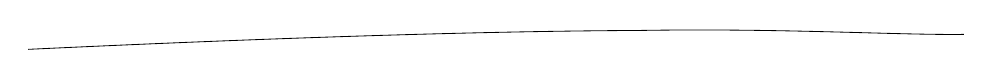
\begin{tikzpicture}[x=\linewidth,y=1mm]
\draw[line width=.3pt] (0,0) .. controls (.21,1.2) and (.45,2.3) .. (.64,2.4) .. controls (.79,2.7) and (.91,1.8) .. (.98,1.9);
\end{tikzpicture}}
\margin{\figure{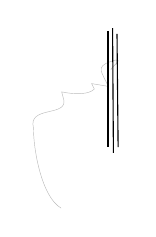
\begin{tikzpicture}[x=1pt,y=1pt]
\draw[black!27,line width=.16pt] (-17,-64) .. controls (-24,-60) and (-27,-43) .. (-27,-35) .. controls (-29,-27) and (-15,-31) .. (-16,-25) -- (-16.8,-22) .. controls (-12,-23) and (-7,-23) .. (-5,-21) -- (-6,-19) -- (0,-20) .. controls (-2,-15) and (-5,-13) .. (1,-11) .. controls (7,-9) and (1,-13) .. (1,-14);
\draw[line width=.65pt] (0,0) -- (0,-42);
\draw (1.6,1) -- (1.9,-44);
\draw (3.2,-1) -- (3.6,-42);
\end{tikzpicture}}}
Finalement, la condition \unsure{irréductible} à imposer à $\mathcal{T}'$ pour la caractériser dans $\underline{\underline{\mathcal{T}}}$, c'est la condition évidente : pour $A\subset \unsure{U|u|n}=S\setminus T$, son adhérence pour $\mathcal{T}$, et pour $\mathcal{T}'$, est la $=$ (ce qui implique déjà $\mathcal{T}\mid U=\mathcal{T}'\mid U$)

Cela donne l'adhérence d'une partie quelconque $A$, comme
\[
\overline{A}^{(\mathcal{T}')}=\overline{A\cap U}^{(\mathcal{T})}\cap\overline{(A\cap T)}^{(\mathcal{T}'_0)}
\]

